\documentclass[psamsfonts,onesided,10pt]{amsart}
\usepackage{goodstyle}


%opening
\title{HW 3 - Write Up}
\author{Robin Belton, Daniel Laden, Jiahui Ma,  Badr Zerktouni}

\begin{document}

\maketitle

\section{System Usage}

This system was written with Python version 3.7 and uses Iris Data csv located at \path{https://github.com/jiahuiblair/CSCI-550/HW3/iris.csv} 
to test clustering and assessment algorithms. All python functions and packages are included in the \path{main.py} file.

All functions can be run in the command line as follows:

\begin{description}
\item[$k$-Nearest Neighbors] To provide classification labels to the testing dataset based on the $k$-nearest neighbors from the training dataset for the Iris data. The input is the Iris data. Then, the users need to specify how large the trainging dataset will be. At last, input training_data, labels, testing data, and number of nearest neighbors into k_nearest function to run the code. The output is a dataframe with both new labels and old labels of the testing data.
\item[Decision Tree] 
\item[$k$ Fold Cross Validation] 
\item[$F$-measure] To compute the $F$-measure of the clustered Iris data, run \textsc{Fmeasure}$(D)$ 
where $D$ is a six-dimensional dataframe with attributes: Sepal Length, Sepal Width, Petal Length, Petal Width,
              Species, and New Label, where the New Label is from the cluster identification. 
\end{description}
 
\section{Example of Input/Output}
\begin{description}
\item[$k$-Nearest Neighbors] \todo{}

\item[Decision Tree] \todo{}

\item[$k$ Fold Cross Validation] \todo{}

\item[$F$-measure] Below we take the output from $k$-nearest neighbors when $k=4$ and then compute the $F$-measure. 
\begin{verbatim}
D = k_nearest(training_data,labels,testing,4)
Fmeasure(D)
# output = 0.9544753086419752
\end{verbatim}
\end{description}

\section{Exploring Datasets}
In this section we describe our findings from Part 4. We explored how varying $k$ affected the output of $k$-nearest neighbors, how applying the clustering algorithms on lower dimensional subsets of the data affected the output, and compared $k$-nearest neighbors to the decision tree on the Iris dataset. 

First, we varied $k$ to see how this parameter affected the output of $k$-nearest neighbors on the Iris dataset. For this particular dataset, we found that even setting $k$ to as low as one gave a high $F$-measure. For $k\in \{1,...,15\}$, we got a high $F$-measure (above .9). However, once $k$ got higher than 15, then $F$-measure dropped significantly or in some cases was not even defined since not many points were being classifed as Iris-setosa. Overall, we were happy with how $k$-nearest neighbors performed in classifying the iris species. Below is a plot of the true classification and the $k$-nearest neighbors classification for $k=4$. 

\begin{figure}[H]
    \centering
    {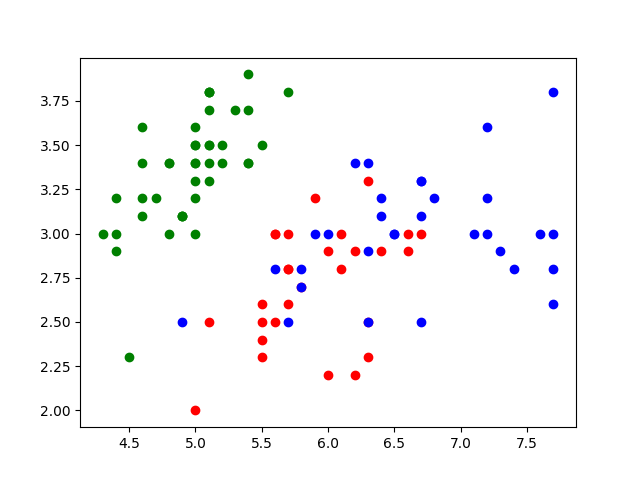
\includegraphics[width=.4\textwidth]{images/trueclass.png}} 
    {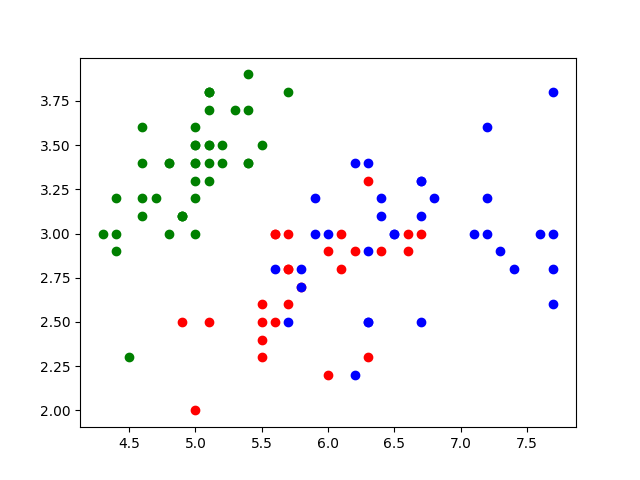
\includegraphics[width=.4\textwidth]{images/KNNclass.png}} 
    \caption{Plots of Sepal Length vs. Sepal Width of the Iris dataset. Left. The true classification of species is indicated by color. Right. Classification of species by $k$-nearest neighbors when $k=4$ is indicated by color. For both plots Versicolor is red, Virginica is blue, and Setosa is green.}
\end{figure}

\todo{finish}

\end{document}
